\section{FTS transfer failures} \label{sec:FTS_failures}


In practice, occasional faults may happen at various levels during data transfers, which may include a wide range of root causes, provoking failures during the shipment of the files.
These errors may vary from naive ones -- e.g. a mistyped command or the request of an unavailable file -- to more severe software and hardware defects.
For instance, the requesting endpoint or archiving server might be temporarily unreachable (connection shortage).
Likewise, the requested data may be corrupted (checksum error) due to storage hardware faults or unstable connection (network problem).
Also, there might be timeouts when the shipment takes more than the pre-configured waiting window -- e.g. when the desired data are bigger than usual and/or must be retrieved from tape, thus requiring more time.
In addition, errors of different nature may often arise due to the interactions between miscellaneous middleware layers.
All of these factors, and more, can generate significant service disruptions and infrastructure malfunctions that require prompt intervention.
For this reason, data transfer processes are continuously monitored by teams of shifters. When an issue is detected, the operators report it through the Global Grid User Support (GGUS) ticketing system \cite{antoni2008ggus}, and experts and site maintainers take care of their solution.
To give an idea of the volumes involved, the ATLAS collaboration alone experienced an average traffic of more than 2 PB per day in 2019 \cite{calafiura2020design_report}, corresponding to roughly 1.5-2 million files moved each day.
Nearly 10\% of these transfers failed producing about 100-200k errors on a daily basis. 
In total, transfer failures generated more than 4k incident reports filed in 2019\footnote{\ggus} for all the LHC experiments (1141 for ATLAS only).
Due to the complexity of the infrastructure and its layered composition, understanding the problem root causes and fixing them demands a great human effort -- more than 100 ATLAS members were involved in 2019, corresponding to roughly 50 FTEs (Full-Time Equivalent)~\cite{jarka2019ftes} -- and it may entail undesired disservices.
The average solving time may vary from a few hours or days -- e.g. in the case of issues that are easy to solve or have already been dealt with in the past -- to entire weeks -- e.g. for unknown problems or more troublesome malfunctions that imply important software or hardware interventions.
In practice, the median solving time for incidents reported by the ATLAS, CMS and LHCb collaborations in 2019 was around 17 days, with a 90\textit{-th} percentile of 44 days and a long right tail extending over 100 days (see \cref{fig:ggus_time}).
\begin{figure}
    \centering
    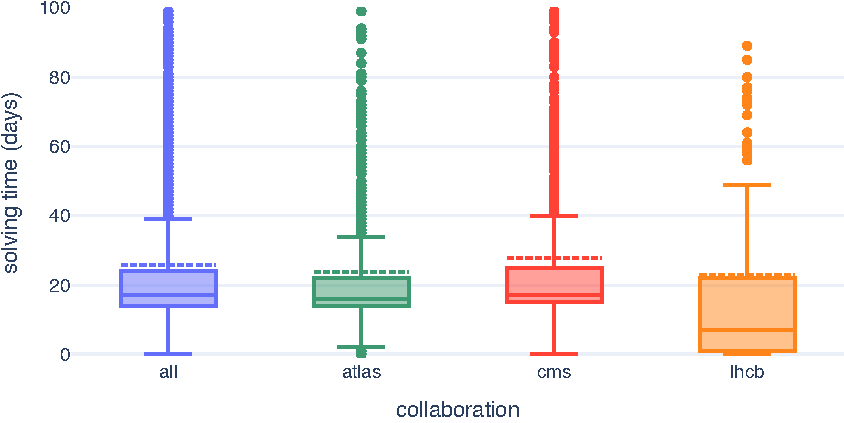
\includegraphics[width=\textwidth]{figures/220_introduction/GGUS_time.pdf}
    \caption{\textbf{Tickets solving time.} Boxplot of the distribution of the solving time for GGUS incidents reported in 2019 by ATLAS, CMS and LHCb collaborations.}
    \label{fig:ggus_time}
\end{figure}
When a transfer failure happens,
the FTS log files are parsed and the transfers more relevant features are extracted and re-organized in a structured format. 
In particular, this involves collecting the exit status of each of the subsystems responsible for the transfer and appending them to compose a global error message.
This information is then exposed to the on-duty shifters along with other characteristics -- e.g. source and destination endpoints, file size, exchange protocol and so on -- and visualizations -- e.g. time evolution plots or site transfer efficiency -- for more in-depth investigations.
% \lc{Here goes some reference to the orders of magnitude at stake, i.e.: 
% \begin{itemize}
%     \item n. tranfers/day (whole or per virtual organization) --> can retrieve from FTS
%     \item ticket/year or month or day (whole or per virtual organization) --> how to retrieve that? is there any official source?
% \end{itemize}
% }

% \lc{Describe current operations and possibly volumes: 
% \begin{itemize}
%     \item Current operations: efficiency matrix + drill down (description + falls)
%     \item average solving time $\rightarrow$ how to retrieve that? is there any official source?
%     \item n. people involved (both shifters and sites) $\rightarrow$ how to retrieve that? is there any official source?
% \end{itemize}
% }
%Current operations are based on a site-centric monitoring approach that involves mainly manual, post-mortem reporting. In this approach, trained operators look at Grafana dashboards that act as a high-level overview of the systems status and try to spot hints of incorrect or undesired behaviours.
Current operations are based on a \textit{site-centric} approach where trained personnel monitors the status of the various services almost 24/7 and tries to spot hints of incorrect or undesired behaviors. In particular, the operators look at Grafana dashboards to get a high-level overview of the system. A usual starting point is the so-called efficiency matrix (\cref{fig:efficiency_matrix}), where the percentage of successful transfers is reported. The granularity level is customizable and it may range from global transfers between national cloud infrastructures involving more computing centers to a finer tracking of particular site exchanges or even specific endpoint links. 
When the efficiency falls below an acceptable threshold, typically 60-70\%, on-duty shifters start to investigate the issue at a lower level by checking \emph{i)} where the error happened, \emph{ii)} how many errors are produced, \emph{iii)} what is the time pattern (temporary, extended or cyclical) and \emph{iv)} which error messages are generated. 
However, this procedure gives rise to many false alarms as it is usual to encounter problems that do not represent a real concern. For instance, this may happen when few transfers are attempted so even a low number of errors imply a high failure rate, or when there are after-effects of a transient issue that had already been fixed. 
Also, sometimes unnecessary drill-down activity is performed for actual issues that were already known, as in the case of ongoing tickets or site downtimes, for which reporting is not required.
As a result, many human resources are employed in repetitive tasks of little scientific interest that would enormously benefit from automation. 

In addition to that, the site-centric strategy described above has some drawbacks. Firstly, monitoring focuses on spotting where issues occur, while understanding the actual root causes is typically demanded to site experts in a subsequent investigation.
Secondly, problems generating few error messages are usually ignored. This is natural, and to some extent desirable, as having limited resources forces us to address bigger malfunctioning first. However, that could be a potential pitfall in cases where promptly fixing a minor issue may prevent the rising of a more significant and longer to solve defect.

All these problems could be tackled programmatically by standardizing the logging output of all the services. In this way, neat error messages would point directly to the source of the problem, thus allowing complete automation. 
However, the distributed nature of the infrastructure hampers such an approach.
In fact, the opportunistic gathering of computing resources that led to WLCG entails many local configurations that are not easy to address using only a static strategy.
Therefore, all these considerations expose the need for an intelligent support tool for speeding up infrastructure management to meet the productivity requirements for the near future.

\begin{landscape}
\begin{figure}
    \centering
    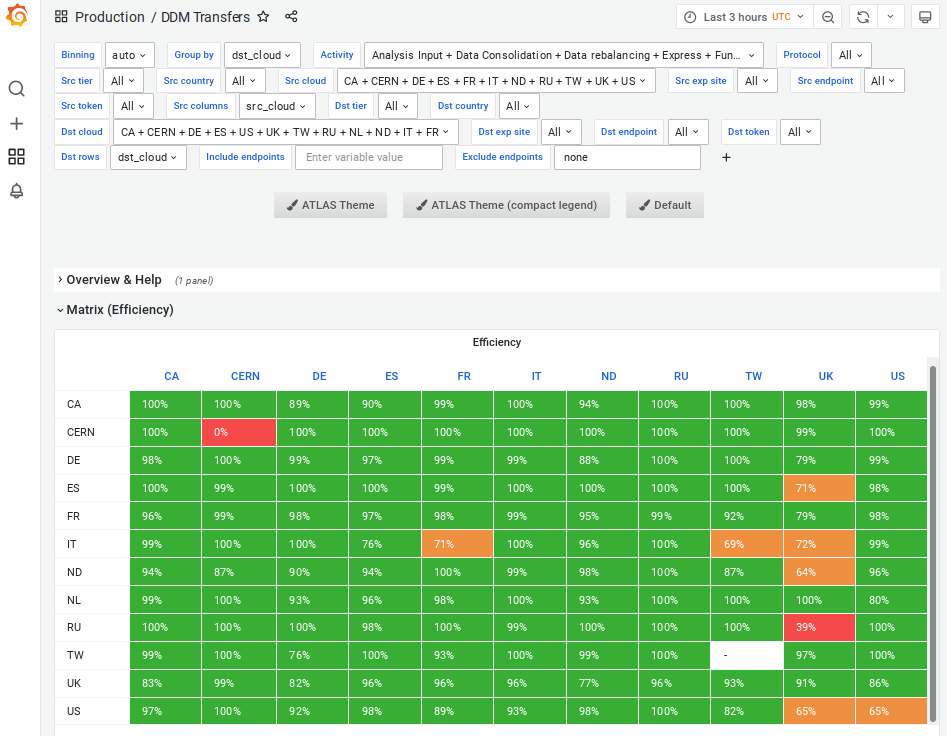
\includegraphics[height=\textwidth]{figures/220_introduction/grafana_efficiency_matrix_narrow1.png}
    \caption{\textbf{Transfer efficiency matrix (Grafana).} Transfer sources are shown as columns and destinations as rows. The drop-down menus at the top allow for custom filtering at the desired level of granularity.}
    \label{fig:efficiency_matrix}
\end{figure}
\end{landscape}